% Provenance (never printed): cycle 2 "Questionner l'espace et le temps"
% (the globe, the continents and the oceans, reading a world map); see
% sources/book1/PROVENANCE.md. Book 1, grade 3, chapter 2.
\chapter{地球仪：大陆与海洋}\label{ch:g3:continents-and-oceans}

在莉娜的教室里，有一个放在支架上的\omterm{def:g3:continents-and-oceans:globe}{地球仪}。莉娜闭上眼睛，
用一根手指把它转起来，再用指尖把它停住。她
睁开眼睛：手指停在蓝色上，正好是在一大片\omterm{def:g2:water-on-earth:ocean}{海洋}的中央。她再试一次：
又是蓝色。第三次，她的手指停在黄绿色上，
位于非洲中部的某个地方。

莉娜继续玩，并数一数。她的手指停在海上的次数
比停在陆地上多得多。为什么呢？还有那些
在她手指下转动的陆地与水域的形状，是什么样的？

\begin{omfigure}
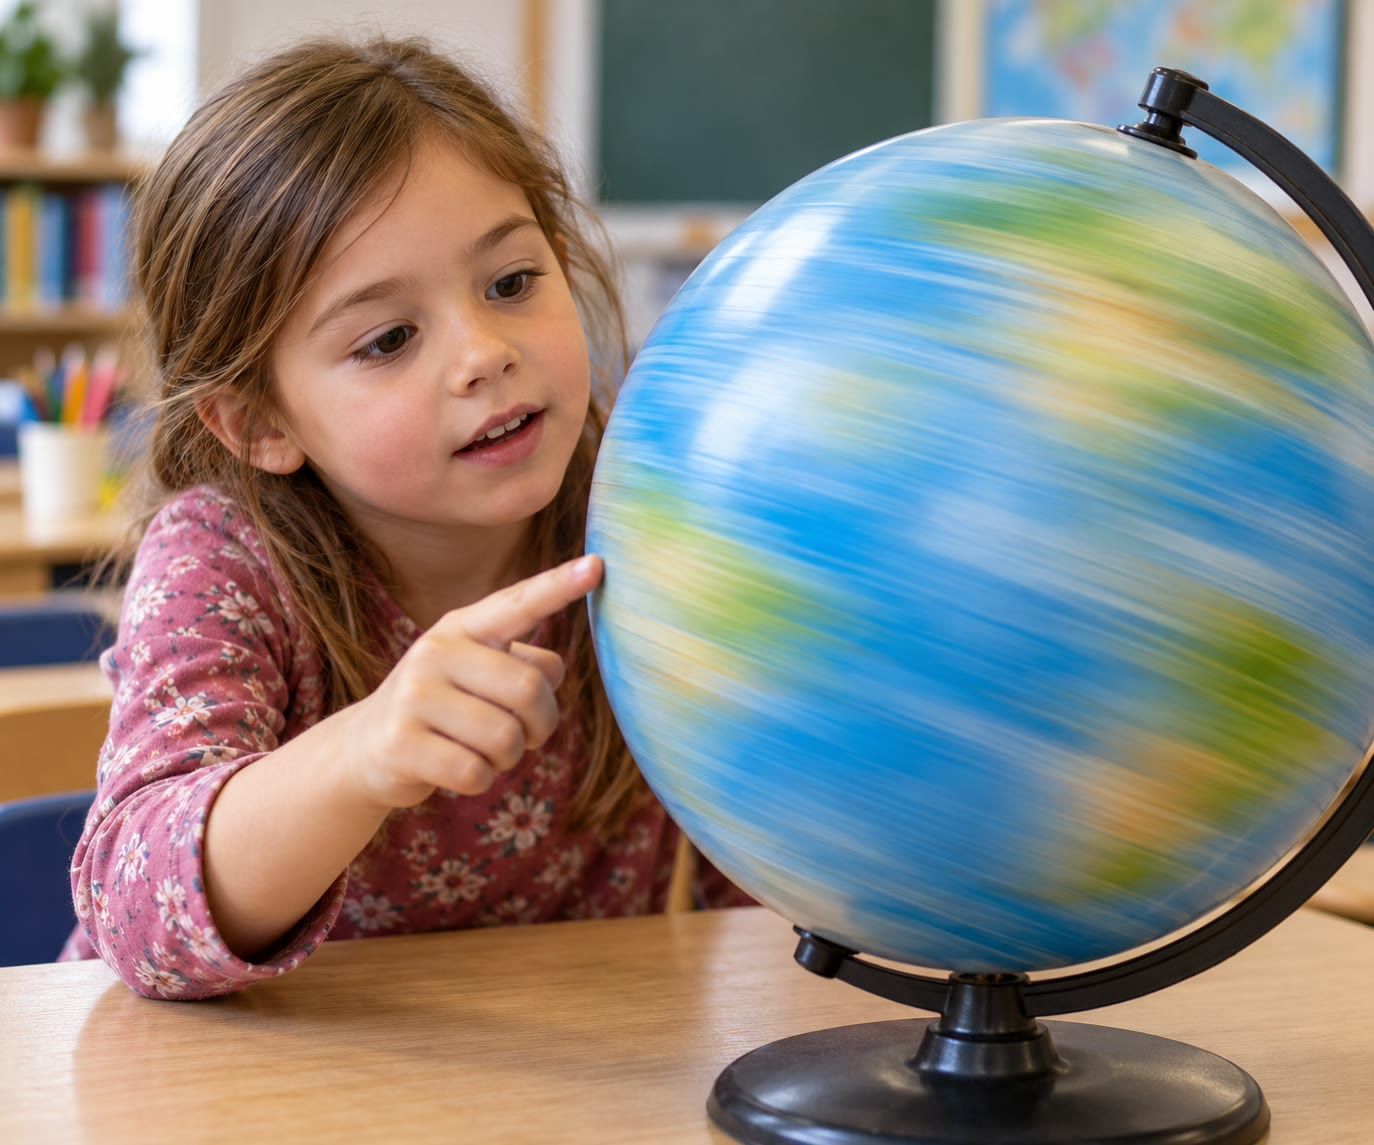
\includegraphics[width=0.6\linewidth]{images/book1/ai/g3-spinning-globe.jpg}

{\small 放在支架上转动的\omterm{def:g3:continents-and-oceans:globe}{地球仪}，陆地与\omterm{def:g2:water-on-earth:ocean}{海洋}
在手指下不断转过。}
\end{omfigure}

\begin{recall}
地球大部分被\omterm{def:g2:water-on-earth:salt-fresh}{咸水}覆盖：在
\cref{ch:g2:water-on-earth}的方格图中，约 71 格（共 100 格）为\omterm{def:g2:water-on-earth:salt-fresh}{咸水}。\omterm{def:g2:water-on-earth:ocean}{海洋}是非常大的一片
\omterm{def:g2:water-on-earth:salt-fresh}{咸水}，位于陆地之间；海是较小的一片，位于
\omterm{def:g2:water-on-earth:ocean}{海洋}的边缘。\omterm{def:g2:drawing-to-map:map}{地图}是从上方看到的地方的缩小画，
（见\cref{ch:g2:drawing-to-map}）。物理课本讲述地球如何
绕自身转动，一天转一圈，由此产生了白天和黑夜。
\end{recall}

\section{地球仪：圆形地球的小模型}

地球是圆的，像一个非常大的球。我们无法从
地面上看清它的形状，因为它太大了：无论站在哪里，
脚下的地面看起来都是平的。但是，飞到离地球很远处的宇航员看到了完整的地球，一个
黑色天空中圆圆的蓝色球体（见
\cref{ch:g2:water-on-earth}开头的照片）。

要在教室里看到整个地球，我们把它缩小。

\begin{definition}[地球仪]\label{def:g3:continents-and-oceans:globe}
称\emph{地球仪}\index{地球仪}为地球的模型：一个
球体，上面按照真实地球的形状画出陆地和\omterm{def:g2:water-on-earth:ocean}{海洋}，
只是小得多。
\end{definition}

\omterm{def:g3:continents-and-oceans:globe}{地球仪}是最好的地球图像，因为它的形状正确：
是圆的。但和真实地球一样，我们每次只能看到
它的一半。要看另一半，就把它转过来。

\begin{omfigure}
\begin{tikzpicture}
\begin{axis}[name=atl, hide axis, axis equal image, scale only axis,
    width=6.2cm, xmin=-1.05, xmax=1.05, ymin=-1.05, ymax=1.05, clip=false]
  \fill[omSea] (axis cs:0,0) circle[radius=1];
  \addplot[fill=omHypsLandA!85!black, draw=black!45, line width=0.2pt]
    table {figdata/out/grade-3-globe-atlantic-land.dat};
  \addplot[black!60, dashed, line width=0.5pt]
    table {figdata/out/grade-3-globe-atlantic-equator.dat};
  \addplot[only marks, mark=*, mark size=1.4pt, black]
    table[x=x, y=y] {figdata/out/grade-3-globe-atlantic-poles.dat};
  \addplot[only marks, mark=none, point meta=explicit symbolic, opacity=0, forget plot]
    table[x=x, y=y, meta=name] {figdata/out/grade-3-globe-atlantic-labels.dat};
  \node[font=\scriptsize, anchor=center, fill=white, fill opacity=0.7, text opacity=1, inner sep=1pt, rounded corners=1pt] at (axis cs:-0.683,0.636) {北美洲};
  \node[font=\scriptsize, anchor=center, fill=white, fill opacity=0.7, text opacity=1, inner sep=1pt, rounded corners=1pt] at (axis cs:-0.561,-0.408) {南美洲};
  \node[font=\scriptsize, anchor=center, fill=white, fill opacity=0.7, text opacity=1, inner sep=1pt, rounded corners=1pt] at (axis cs:0.396,0.639) {欧洲};
  \node[font=\scriptsize, anchor=center, fill=white, fill opacity=0.7, text opacity=1, inner sep=1pt, rounded corners=1pt] at (axis cs:0.704,-0.098) {非洲};
  \node[font=\scriptsize, anchor=center, fill=white, fill opacity=0.7, text opacity=1, inner sep=1pt, rounded corners=1pt] at (axis cs:-0.209,0.128) {大西洋};
  \draw[black!70, line width=0.8pt] (axis cs:0,0) circle[radius=1];
  \node[font=\scriptsize, anchor=south] at (axis cs:0,0.97) {北极};
\end{axis}
\begin{axis}[at={(atl.east)}, anchor=west, xshift=0.6cm, hide axis,
    axis equal image, scale only axis,
    width=6.2cm, xmin=-1.05, xmax=1.05, ymin=-1.05, ymax=1.05, clip=false]
  \fill[omSea] (axis cs:0,0) circle[radius=1];
  \addplot[fill=omHypsLandA!85!black, draw=black!45, line width=0.2pt]
    table {figdata/out/grade-3-globe-pacific-land.dat};
  \addplot[black!60, dashed, line width=0.5pt]
    table {figdata/out/grade-3-globe-pacific-equator.dat};
  \addplot[only marks, mark=none, point meta=explicit symbolic, opacity=0, forget plot]
    table[x=x, y=y, meta=name] {figdata/out/grade-3-globe-pacific-labels.dat};
  \node[font=\scriptsize, anchor=center, fill=white, fill opacity=0.7, text opacity=1, inner sep=1pt, rounded corners=1pt] at (axis cs:-0.754,-0.391) {澳大利亚};
  \node[font=\scriptsize, anchor=center, fill=white, fill opacity=0.7, text opacity=1, inner sep=1pt, rounded corners=1pt] at (axis cs:0.258,0.087) {太平洋};
  \draw[black!70, line width=0.8pt] (axis cs:0,0) circle[radius=1];
\end{axis}
\end{tikzpicture}

{\small 从两侧看\omterm{def:g3:continents-and-oceans:globe}{地球仪}。左图：大西洋
一侧，包括美洲、欧洲和非洲。右图：另一侧，
即太平洋一侧，澳大利亚位于其边缘。虚线为\omterm{def:g3:continents-and-oceans:equator}{赤道}。
\omterm{def:g1:landscapes-around-us:water}{海岸}线：Natural Earth（公有领域）。}
\label{fig:g3:continents-and-oceans:globes}
% ledger: data:ne-land
\end{omfigure}

\begin{remark}[两个截然不同的半球]\label{rem:g3:continents-and-oceans:halves}
看看这两幅图。在左图中，陆地约占
10 份中的 4 份；在右图中，只占约 10 份中的 1 份：地球的太平洋一侧
几乎全是水。如果莉娜的手指停在\omterm{def:g3:continents-and-oceans:globe}{地球仪}的那一侧，
几乎总会停在海上。
\end{remark}

\section{赤道、两极与两个半球}

\omterm{def:g3:continents-and-oceans:globe}{地球仪}绕着一根贯穿其中、从顶端到底端的轴杆转动。
真实的地球没有轴杆，但它也绕着穿过
其中心的一条线转动。这条线穿出地球的两个地方都有名称。

\begin{definition}[极]\label{def:g3:continents-and-oceans:poles}
称\emph{北极}\index{北极}和\emph{南
极}\index{南极}为地球最顶端和最底端的两个点，
即地球绕其转动的那条线穿出的地方。它们中的每一个都是
\emph{极}\index{极}。在\omterm{def:g3:continents-and-oceans:globe}{地球仪}上，北极位于
最上方。
\end{definition}

\begin{definition}[赤道与半球]\label{def:g3:continents-and-oceans:equator}
\emph{赤道}\index{赤道}是一条假想的线，
绕地球一周，恰好位于\omterm{def:g3:continents-and-oceans:poles}{北极}和\omterm{def:g3:continents-and-oceans:poles}{南极}的正中间。
它把地球分成两半，每一半都称为一个
\emph{半球}\index{半球}：\emph{北半球}\index{北半球}，
位于\omterm{def:g3:continents-and-oceans:poles}{北极}一侧，
另一半是\emph{南半球}\index{南半球}，
位于\omterm{def:g3:continents-and-oceans:poles}{南极}一侧。
\end{definition}

\omterm{def:g3:continents-and-oceans:equator}{赤道}并没有画在地面上：在海滩或森林里，
谁也看不见它。它画在\omterm{def:g3:continents-and-oceans:globe}{地球仪}和\omterm{def:g2:drawing-to-map:map}{地图}上，帮助我们找路。

\begin{omfigure}
\begin{tikzpicture}[font=\small]
  % globe outline
  \fill[omSea!70] (0,0) circle (2.2);
  % northern hemisphere tinted
  \begin{scope}
    \clip (0,0) circle (2.2);
    \fill[yellow!25, opacity=0.8] (-2.3,0) -- (-2.3,2.3) -- (2.3,2.3) -- (2.3,0)
      arc[start angle=0, end angle=-180, x radius=2.3, y radius=0.45] -- cycle;
  \end{scope}
  \draw[black!70, line width=0.8pt] (0,0) circle (2.2);
  % equator: front half solid, back half dashed
  \draw[red!70!black, line width=1.2pt] (-2.2,0) arc[start angle=180, end angle=360, x radius=2.2, y radius=0.4];
  \draw[red!70!black, line width=0.8pt, dashed] (2.2,0) arc[start angle=0, end angle=180, x radius=2.2, y radius=0.4];
  % axis and poles
  \draw[black!60, line width=0.6pt] (0,2.2) -- (0,2.75);
  \draw[black!60, line width=0.6pt] (0,-2.2) -- (0,-2.75);
  \draw[black!60, line width=0.6pt, dotted] (0,2.2) -- (0,-2.2);
  \fill (0,2.2) circle (2.2pt);
  \fill (0,-2.2) circle (2.2pt);
  \node[anchor=west] at (0.15,2.6) {北极};
  \node[anchor=west] at (0.15,-2.6) {南极};
  % labels
  \node[anchor=west] at (2.6,0) {赤道};
  \draw[black!60] (2.55,0) -- (2.05,-0.15);
  \node[anchor=west, align=left] at (2.6,1.4) {北半球};
  \draw[black!60] (2.55,1.4) -- (1.5,1.2);
  \node[anchor=west, align=left] at (2.6,-1.4) {南半球};
  \draw[black!60] (2.55,-1.4) -- (1.5,-1.2);
\end{tikzpicture}

{\small \omterm{def:g3:continents-and-oceans:equator}{赤道}把地球分成两个\omterm{def:g3:continents-and-oceans:equator}{半球}。
\omterm{def:g3:continents-and-oceans:equator}{北半球}（着色部分）位于\omterm{def:g3:continents-and-oceans:poles}{北极}一侧，\omterm{def:g3:continents-and-oceans:equator}{南半球}
位于\omterm{def:g3:continents-and-oceans:poles}{南极}一侧。}
\label{fig:g3:continents-and-oceans:hemispheres}
\end{omfigure}

\begin{example}[赤道附近炎热，两极附近寒冷]\label{ex:g3:continents-and-oceans:hot-cold}
\omterm{def:g3:continents-and-oceans:equator}{赤道}附近的陆地全年都很炎热：这里
正是大片雨林生长的地方。两极附近的陆地全年都很寒冷，
大部分被冰雪覆盖。这一现象的原因
你将在以后学到。现在请记住：离两极越近，就越冷。
\end{example}

\section{七大洲和五大洋}

在\omterm{def:g3:continents-and-oceans:globe}{地球仪}上，陆地并不是到处散布成小块，
大部分陆地集中在少数几个非常大的陆块中。

\begin{definition}[大陆]\label{def:g3:continents-and-oceans:continent}
\emph{大陆}\index{大陆}是地球上非常大的陆块之一，
连同靠近它的岛屿。
\end{definition}

人们最常说的是七大洲。按由大到小的顺序，
它们依次是：亚洲、非洲、北美洲、南美洲、\omterm{def:g3:continents-and-oceans:poles}{南极}洲、欧洲、
以及澳大利亚。
% ledger: natgeo:seven-continents

\begin{center}\small
\begin{tabular}{rlll}
\hline
排名 & 大洲 & 所在\omterm{def:g3:continents-and-oceans:equator}{半球} & 说明 \\
\hline
1 & 亚洲 & 大部分在\omterm{def:g3:continents-and-oceans:equator}{北半球} & 最大 \\
2 & 非洲 & 南\omterm{def:g3:continents-and-oceans:equator}{北半球}都有 & \omterm{def:g3:continents-and-oceans:equator}{赤道}穿过其中部 \\
3 & 北美洲 & \omterm{def:g3:continents-and-oceans:equator}{北半球} & 向北延伸得很远 \\
4 & 南美洲 & 大部分在\omterm{def:g3:continents-and-oceans:equator}{南半球} & \omterm{def:g3:continents-and-oceans:equator}{赤道}穿过其北部 \\
5 & \omterm{def:g3:continents-and-oceans:poles}{南极}洲 & \omterm{def:g3:continents-and-oceans:equator}{南半球} & 环绕\omterm{def:g3:continents-and-oceans:poles}{南极}，被冰层覆盖 \\
6 & 欧洲 & \omterm{def:g3:continents-and-oceans:equator}{北半球} & 东侧与亚洲相连 \\
7 & 澳大利亚 & \omterm{def:g3:continents-and-oceans:equator}{南半球} & 最小 \\
\hline
\end{tabular}
\end{center}

\begin{remark}[一块大陆在哪里结束？]\label{rem:g3:continents-and-oceans:where}
有些\omterm{def:g3:continents-and-oceans:continent}{大陆}四周都被\omterm{def:g2:water-on-earth:ocean}{海洋}环绕，如澳大利亚
或\omterm{def:g3:continents-and-oceans:poles}{南极}洲。另一些则相连：欧洲与亚洲是同一块陆地，
人们选择在两者之间划定界线，因此有些人
只数六大洲，甚至更少。
\end{remark}

大洲之间是\omterm{def:g2:water-on-earth:ocean}{海洋}，共有五个。其中最大的
是\emph{太平洋}；其后是\emph{大西洋}、
\emph{印度洋}、环绕\omterm{def:g3:continents-and-oceans:poles}{南极}洲的\emph{南大洋}，以及
最小的、环绕\omterm{def:g3:continents-and-oceans:poles}{北极}的\emph{北冰洋}。很长一段时间里，
人们只数四个；如今大多数国家将南大洋
算作第五个。
% ledger: nos:five-oceans, nos:pacific-largest, oer:arctic-smallest

\begin{example}[太平洋有多大？]\label{ex:g3:continents-and-oceans:pacific}
太平洋非常辽阔，把所有大洲放在一起，
也放得进去。它所含的海水超过全球海水的一半，
这就是本章第一节中右边的\omterm{def:g3:continents-and-oceans:globe}{地球仪}看上去
几乎全是蓝色的原因。
% ledger: nos:pacific-largest
\end{example}

\begin{method}[找出两块大陆之间的大洋]\label{met:g3:continents-and-oceans:between}
要找出两块\omterm{def:g3:continents-and-oceans:continent}{大陆}之间是哪一片大洋，先在\omterm{def:g3:continents-and-oceans:globe}{地球仪}上为每块\omterm{def:g3:continents-and-oceans:continent}{大陆}各按一根手指，
再转动\omterm{def:g3:continents-and-oceans:globe}{地球仪}，使两根手指都能看到。
眼睛从一根手指移到另一根手指所经过的大洋，就是两者之间的大洋。
\omterm{def:g3:continents-and-oceans:globe}{地球仪}上常有两条路可走：选择较短的那条。
\end{method}

\begin{example}[非洲与澳大利亚]\label{ex:g3:continents-and-oceans:africa-australia}
从非洲向东前往澳大利亚，要穿过印度洋。从
欧洲向西前往北美洲，要穿过大西洋。从亚洲向东
前往北美洲，要穿过太平洋。
\end{example}

\section{世界地图是压平的地球仪}

\omterm{def:g3:continents-and-oceans:globe}{地球仪}是圆的，不易携带，而且我们永远无法一次看到它的全部。
一张纸上的\omterm{def:g2:drawing-to-map:map}{地图}，却能让人一眼看到整个地球。

\begin{definition}[世界地图]\label{def:g3:continents-and-oceans:world-map}
\emph{世界地图}\index{世界地图}是把整个地球平铺在纸上或屏幕上的\omterm{def:g2:drawing-to-map:map}{地图}，
图中同时画出
所有大洲和所有大洋。
\end{definition}

\begin{omfigure}
\begin{tikzpicture}
\begin{axis}[ommap, width=\linewidth, xtick=\empty, ytick={0},
    yticklabels={赤道}, grid=none, clip=true]
  \addplot[fill=omHypsLandA!85!black, draw=black!45, line width=0.2pt]
    table {figdata/out/shared-geo-land.dat};
  \draw[black!60, dashed, line width=0.5pt] (axis cs:-180,0) -- (axis cs:180,0);
  \begin{scope}[every node/.style={font=\scriptsize, align=center}]
    \node at (axis cs:-102,47) {北 \\美洲};
    \node at (axis cs:-60,-12) {南 \\美洲};
    \node at (axis cs:17,52) {欧洲};
    \node at (axis cs:20,6) {非洲};
    \node at (axis cs:92,48) {亚洲};
    \node at (axis cs:134,-24) {澳大利亚};
    \node at (axis cs:40,-80) {南极洲};
  \end{scope}
  \begin{scope}[every node/.style={font=\scriptsize\itshape, align=center, text=omSea!35!black}]
    \node at (axis cs:-145,8) {太平 \\洋};
    \node at (axis cs:165,12) {太平 \\洋};
    \node at (axis cs:-38,22) {大西 \\洋};
    \node at (axis cs:-15,-25) {大西 \\洋};
    \node at (axis cs:78,-22) {印度 \\洋};
    \node at (axis cs:-115,-57) {南大洋};
    \node at (axis cs:-150,79) {北冰洋};
  \end{scope}
\end{axis}
\end{tikzpicture}

{\small 一幅\omterm{def:g3:continents-and-oceans:world-map}{世界地图}。\omterm{def:g3:continents-and-oceans:globe}{地球仪}沿穿过太平洋中部的一条线剪开并摊平：
太平洋出现了两次，分别在左边缘和右边缘。
\omterm{def:g3:continents-and-oceans:poles}{南极}洲是围绕\omterm{def:g3:continents-and-oceans:poles}{南极}的圆形\omterm{def:g3:continents-and-oceans:continent}{大陆}，
在\omterm{def:g2:drawing-to-map:map}{地图}底部被拉伸成一条长带。
\omterm{def:g1:landscapes-around-us:water}{海岸}线数据：Natural Earth（公有领域）。}
\label{fig:g3:continents-and-oceans:world-map}
% ledger: data:ne-land
\end{omfigure}

但这里有一个困难。试着把橙子皮铺在桌上：
它不撕破或拉伸就无法平放。地球表面被画成平面时也是如此。
每一幅\omterm{def:g3:continents-and-oceans:world-map}{世界地图}，都要在某处撕开地球，
或者拉伸某些地方、挤压另一些地方。

\begin{omfigure}
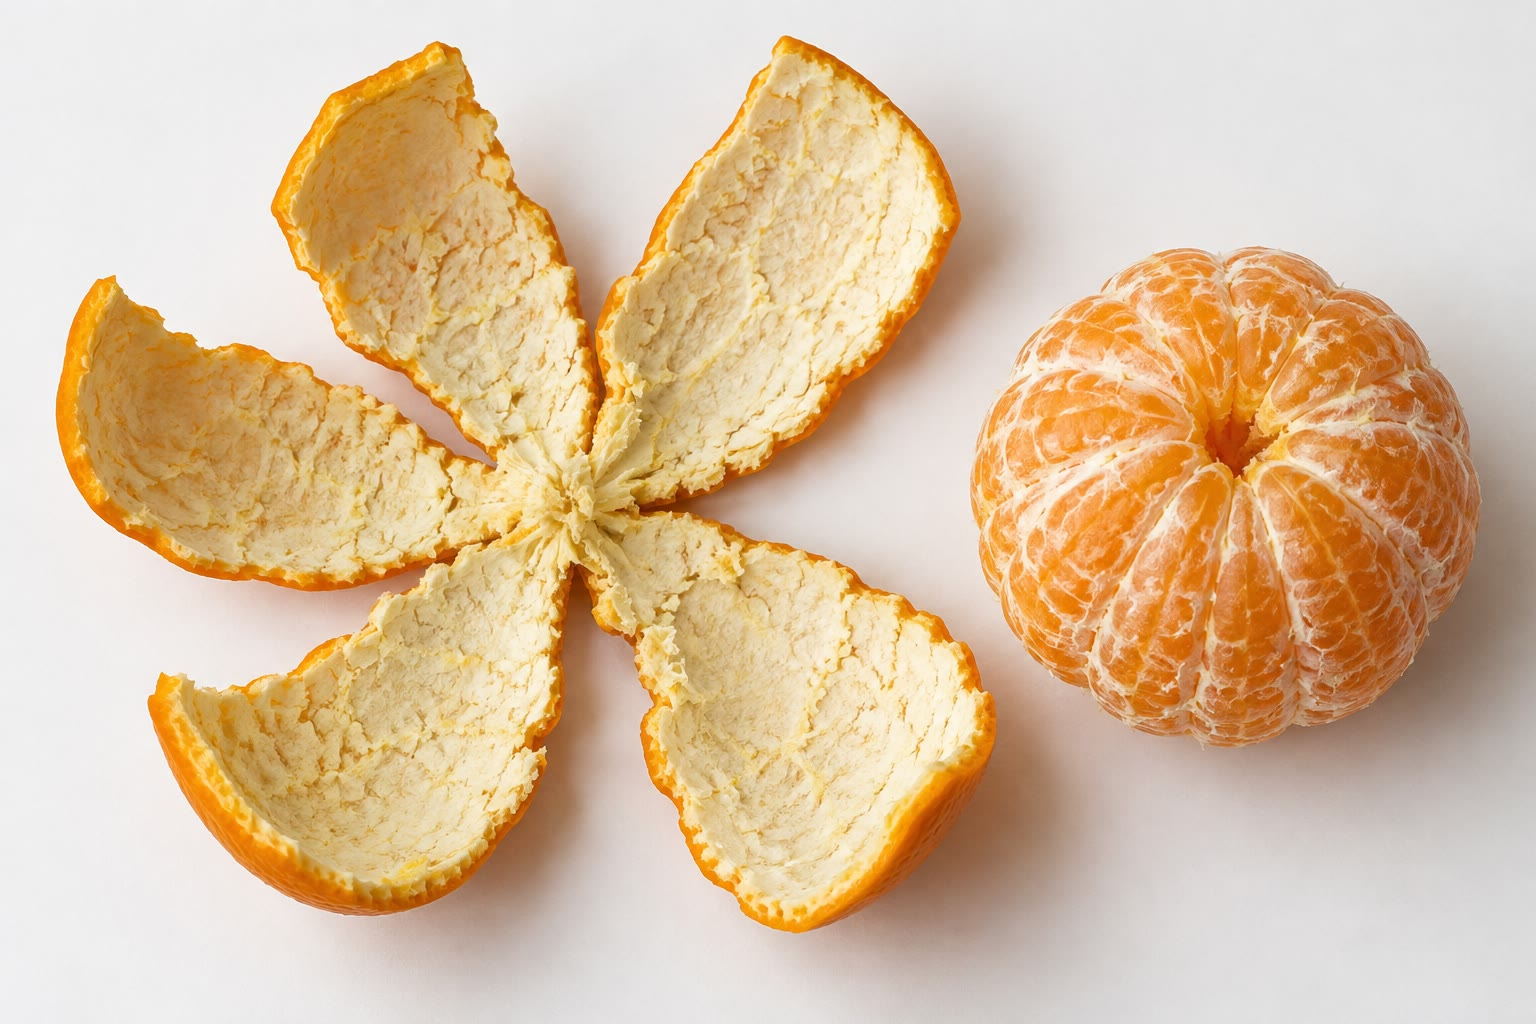
\includegraphics[width=0.4\linewidth]{images/book1/ai/g3-orange-peel.jpg}

{\small 橙子皮不撕破就无法平放。}
\end{omfigure}

\begin{remark}[地图与地球仪并不一致]\label{rem:g3:continents-and-oceans:disagree}
在这幅\omterm{def:g3:continents-and-oceans:world-map}{世界地图}上，\omterm{def:g3:continents-and-oceans:poles}{南极}洲看上去是最大的\omterm{def:g3:continents-and-oceans:continent}{大陆}之一，沿着整个底边被拉长。
在\omterm{def:g3:continents-and-oceans:globe}{地球仪}上，它是一块圆形陆地，比南美洲还小。
靠近两极时，平面\omterm{def:g2:drawing-to-map:map}{地图}把陆地拉伸得很厉害；
靠近\omterm{def:g3:continents-and-oceans:equator}{赤道}时，拉伸得很少。
要比较远离\omterm{def:g3:continents-and-oceans:equator}{赤道}的两个地方的大小，
应以\omterm{def:g3:continents-and-oceans:globe}{地球仪}为准。
\end{remark}

\begin{method}[读世界地图]\label{met:g3:continents-and-oceans:reading}
在这样的\omterm{def:g3:continents-and-oceans:world-map}{世界地图}上：
\begin{enumerate}
  \item 北在上方，南在下方，\omterm{def:g3:continents-and-oceans:poles}{北极}是
        整个上边缘，\omterm{def:g3:continents-and-oceans:poles}{南极}是整个下边缘；
  \item \omterm{def:g3:continents-and-oceans:equator}{赤道}是中间的横线：
        \omterm{def:g3:continents-and-oceans:equator}{赤道}以上的全部位于\omterm{def:g3:continents-and-oceans:equator}{北半球}，
        \omterm{def:g3:continents-and-oceans:equator}{赤道}以下的全部位于\omterm{def:g3:continents-and-oceans:equator}{南半球}；
  \item 左右两边缘在\omterm{def:g3:continents-and-oceans:globe}{地球仪}上是同一条线：
        从右边缘驶出的船，会从左边缘回来。
\end{enumerate}
\end{method}

\section{练习}

\begin{exercise}[$\star$]\label{exo:g3:continents-and-oceans:1}
说出七大洲的名称。哪一个最大？哪一个最小？
\end{exercise}

\begin{exercise}[$\star$]\label{exo:g3:continents-and-oceans:2}
说出五大洋的名称。哪一个最大？哪一个最小？
\end{exercise}

\begin{exercise}[$\star$]\label{exo:g3:continents-and-oceans:3}
抄写并填空，可选“\omterm{def:g3:continents-and-oceans:poles}{北极}”“\omterm{def:g3:continents-and-oceans:poles}{南极}”或“\omterm{def:g3:continents-and-oceans:equator}{赤道}”：
\dots{}在\omterm{def:g3:continents-and-oceans:globe}{地球仪}的顶部；\dots{}在底部；\dots{}
绕着中间一整圈。
\end{exercise}

\begin{exercise}[$\star$]\label{exo:g3:continents-and-oceans:4}
\omterm{def:g3:continents-and-oceans:equator}{北半球}还是\omterm{def:g3:continents-and-oceans:equator}{南半球}？欧洲；澳大利亚；
\omterm{def:g3:continents-and-oceans:poles}{南极}洲；北美洲。
\end{exercise}

\begin{exercise}[$\star$]\label{exo:g3:continents-and-oceans:5}
哪个大洋环绕\omterm{def:g3:continents-and-oceans:poles}{北极}？
哪个大洋环绕\omterm{def:g3:continents-and-oceans:poles}{南极}洲？
\end{exercise}

\begin{exercise}[$\star\star$]\label{exo:g3:continents-and-oceans:6}
从非洲到南美洲，要穿过哪个大洋？从
澳大利亚向东到南美洲呢？从非洲到澳大利亚呢？
\end{exercise}

\begin{exercise}[$\star\star$]\label{exo:g3:continents-and-oceans:7}
萨姆住在一个全年都很热的国家。博住在
一个全年严寒的科考站上。两人中一个住在
\omterm{def:g3:continents-and-oceans:equator}{赤道}附近，另一个住在靠近某个极地的地方。谁住在哪里？
\end{exercise}

\begin{exercise}[$\star\star$]\label{exo:g3:continents-and-oceans:8}
莉娜把\omterm{def:g3:continents-and-oceans:globe}{地球仪}转了 10 次，她的手指有 7 次
落在海上。她的手指有多少次落在陆地上？这和你预想的一样吗？为什么？
\end{exercise}

\begin{exercise}[$\star\star$]\label{exo:g3:continents-and-oceans:9}
在第~\pageref{fig:g3:continents-and-oceans:world-map}~页的\omterm{def:g3:continents-and-oceans:world-map}{世界地图}上，
太平洋出现了两次。为什么？真实的地球上
有两个太平洋吗？
\end{exercise}

\begin{exercise}[$\star\star\star$]\label{exo:g3:continents-and-oceans:10}
汤姆说：“在\omterm{def:g3:continents-and-oceans:world-map}{世界地图}上，\omterm{def:g3:continents-and-oceans:poles}{南极}洲比亚洲长，所以
\omterm{def:g3:continents-and-oceans:poles}{南极}洲是最大的\omterm{def:g3:continents-and-oceans:continent}{大陆}。”汤姆说得对吗？
利用各\omterm{def:g3:continents-and-oceans:continent}{大陆}从大到小的排列，说明\omterm{def:g3:continents-and-oceans:world-map}{世界地图}为什么会误导他。
\end{exercise}
